\documentclass[tikz,border=10pt]{standalone}
\begin{document}

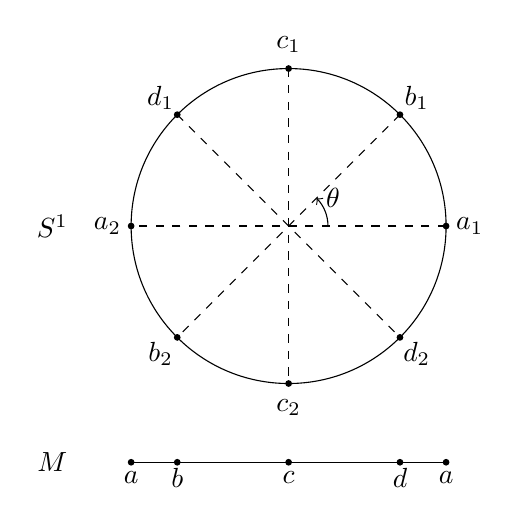
\begin{tikzpicture}

% 绘制圆
\draw (0,0) circle(2);

% 绘制直线
\draw[-] (-2,-3) -- (2,-3);
\draw[->] (0.5,0)arc[start angle = 0, end angle = 45,radius = 0.5] node[right] {$\theta$};
% 标记圆上的点(每隔45°,用字母a, b, c, d, e, f, g, h)
\foreach \angle/\label in {0/$a_1$, 45/$b_1$, 90/$c_1$, 135/$d_1$, 180/$a_2$, 225/$b_2$, 270/$c_2$, 315/$d_2$} {
  \draw[fill] (\angle:2) circle(1pt);
    \node at (\angle:2.3) {\label};
}
\foreach \angle/\label in{0/$a$,-45/$d$, -90/ $c$, -135/ $b$,-180/$a$}{
  \draw[fill] ({2*cos(\angle)},-3) circle(1pt); 
  \node at ({2*cos(\angle)},-3.2){\label};
}
\foreach \angle in {0,45,90,135}{
\draw[dashed] ({2*cos(\angle)},{2*sin(\angle)}) -- ({2*cos(\angle + 180)},{2*sin(\angle+180)});
}
\node at (-3,-3) {$M$};
\node at (-3,0) {$S^1$};
\end{tikzpicture}
\end{document}
